\documentclass{article}
\usepackage{fancyhdr}
\usepackage{ctex}
\usepackage{listings}
\usepackage{graphicx}
\usepackage[a4paper, body={18cm,22cm}]{geometry}
\usepackage{amsmath,amssymb,amstext,wasysym,enumerate,graphicx}
\usepackage{float,abstract,booktabs,indentfirst,amsmath}
\usepackage{array}
\usepackage{booktabs}
\usepackage{multirow}
\usepackage{url}
\usepackage{diagbox}
\renewcommand\arraystretch{1.4}
\usepackage{indentfirst}
\setlength{\parindent}{2em}
\usepackage{enumitem}
\setmonofont{Consolas}
\usepackage{listings}
\usepackage{xcolor}
\usepackage{makecell}
\usepackage{tikz}
\usetikzlibrary{positioning, arrows.meta}
\setCJKmonofont{黑体}
\lstset{  
	% 基本设置  
	xleftmargin = 3em, xrightmargin = 3em, aboveskip = 1em,  
	backgroundcolor = \color{white},  
	basicstyle = \small\ttfamily,  
	rulesepcolor = \color{gray},  
	breaklines = true,  
	numbers = left,  
	numberstyle = \small,  
	numbersep = -14pt,  
	frame = shadowbox,  
	showspaces = false,  
	columns = fixed,  
	sensitive = true,  
	% VSCode 风格配色  
	keywordstyle = \color{blue!70!black}\bfseries,  
	emphstyle = \color{red!70!black}\bfseries, % 对于强调的词  
	emphstyle=[2]\color{purple!70!black}\bfseries, % 对于第二组强调的词  
	commentstyle = \color{green!60!black}, % 注释颜色  
	stringstyle = \color{orange!90!black}, % 字符串颜色更亮一些  
	morekeywords={ASSERT, int64\_t, uint32\_t},  
	moreemph={ASSERT, NULL},  
	moreemph=[2]{int64\_t, uint32\_t, tid\_t, uint8\_t, int16\_t, uint16\_t, int32\_t, size\_t, bool},  
	morecomment=[l][\color{green!60!black}]{+}, % 以+开头的注释  
}

%--------------------页眉--------------------%
\pagestyle{fancy}
\fancyhead[L]{}
\fancyhead[R]{}
\fancyhead[C]{华东师范大学软件工程学院实验报告}
\fancyfoot[C]{-\thepage-}
\renewcommand{\headrulewidth}{1.5pt}
%--------------------标题--------------------%
\begin{document}
\begin{center}
	{\Large{\textbf{\heiti 华东师范大学软件工程学院实验报告}}}
	\begin{table}[H]
		\centering
		\begin{tabular}{p{2cm}p{4cm}<{\centering}p{1cm}p{2cm}p{6cm}<{\centering}}
			课程名称:    & 操作系统实践 & \quad & 指导教师:    & 张民
			\\ \cline{2-2} \cline{5-5}
			姓\qquad 名: & 王海生    & \quad & 学\qquad 号: & 10235101559         \\ \cline{2-2} \cline{5-5}
			实验编号:    & 实验三 & \quad & 实验名称:    & 修改alarm-priority
			\\ \cline{2-2} \cline{5-5}
		\end{tabular}
	\end{table}
	
	% 添加新行并居中
	%\vspace{1em} % 可选:添加垂直间距
	\textbf{代码仓库:}\url{https://github.com/Hanson-Wang-chn/ECNU-Operating-System-WHS.git}
\end{center}
\rule{\textwidth}{1pt}
%--------------------正文--------------------%
\section{实验目的}

\begin{enumerate}[noitemsep, label={{\arabic*})}]
  \item 熟悉PintOS源代码结构
  \item 添加hello-world函数并编译输出
  \item 修改批处理文件实现自动化结果测试
  \item 熟悉\texttt{Visual Studio Code}和\texttt{Git}的使用
\end{enumerate}

\normalsize

\section{实验内容与设计思想}

\normalsize

\section{使用环境}

\subsection{主机系统配置}

本次实验的主机系统环境如下表所示:

\begin{center}
	\begin{tabular}{| >{\centering\arraybackslash}m{3cm} | >{\centering\arraybackslash}m{7cm} |}    
		\hline  
		\textbf{项目名称} & \textbf{详细信息} \\
		\hline  
		操作系统 & macOS Sequoia 15.0 \\  
		\hline  
		系统类型 & 64位操作系统,基于ARM的处理器 \\  
		\hline
		CPU & Apple M1 Pro \\  
		\hline 
		GPU & Apple M1 Pro\\  
		\hline 
		内存 & 16GB 统一内存 \\  
		\hline 
		磁盘 & 512GB SSD \\  
		\hline 		
	\end{tabular}
\end{center}

\subsection{Docker配置}

在官网下载并安装后,Docker容器正常运行,如下图所示:

\begin{figure}[H]
	\centering
	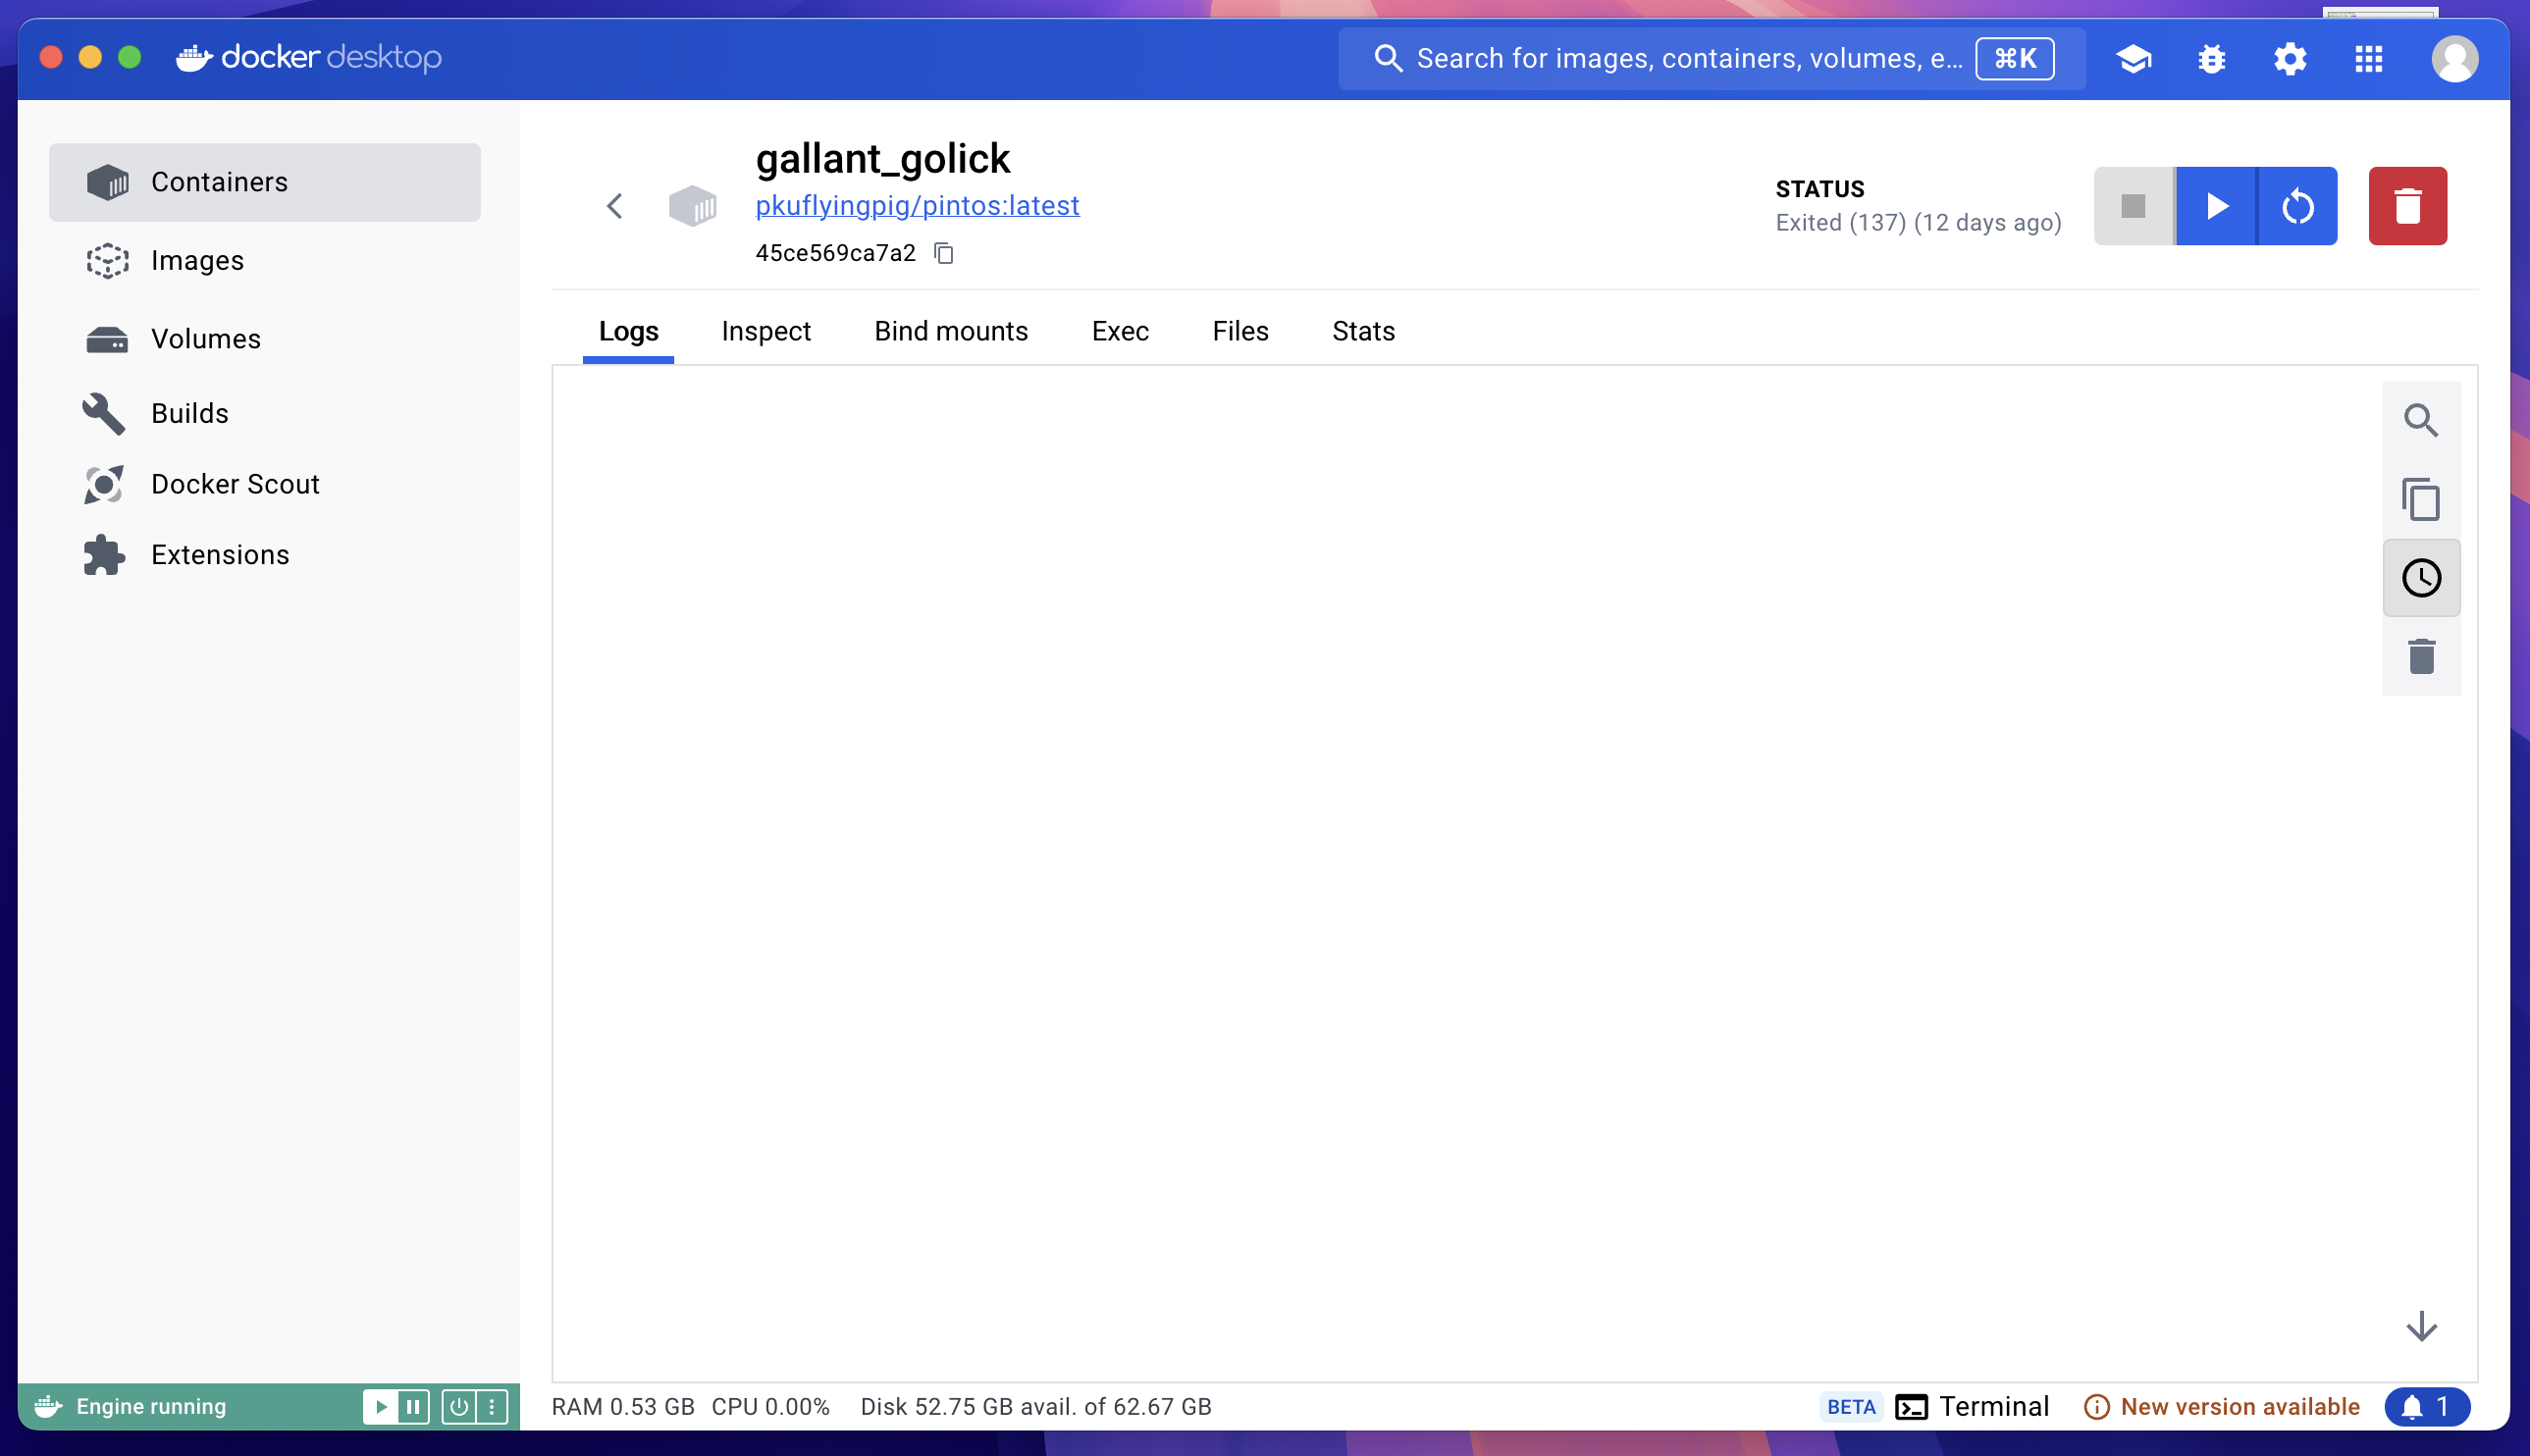
\includegraphics[width=0.9\textwidth]{img/docker_install.png}
	\caption{Docker容器}
\end{figure}

接着使用下面的命令实现磁盘挂载,方便文件管理:

\begin{lstlisting}[language=Bash, title=启动Docker容器并挂载文件]
	docker run -it --rm --name pintos --mount type=bind,\
	source=/Users/wanghaisheng/Desktop/Coding/ECNU-Operating-System-WHS/pintos,\
	target=/home/PKUOS/pintos pkuflyingpig/pintos bash
\end{lstlisting}

完成后如下图所示:

\begin{figure}[H]
	\centering
	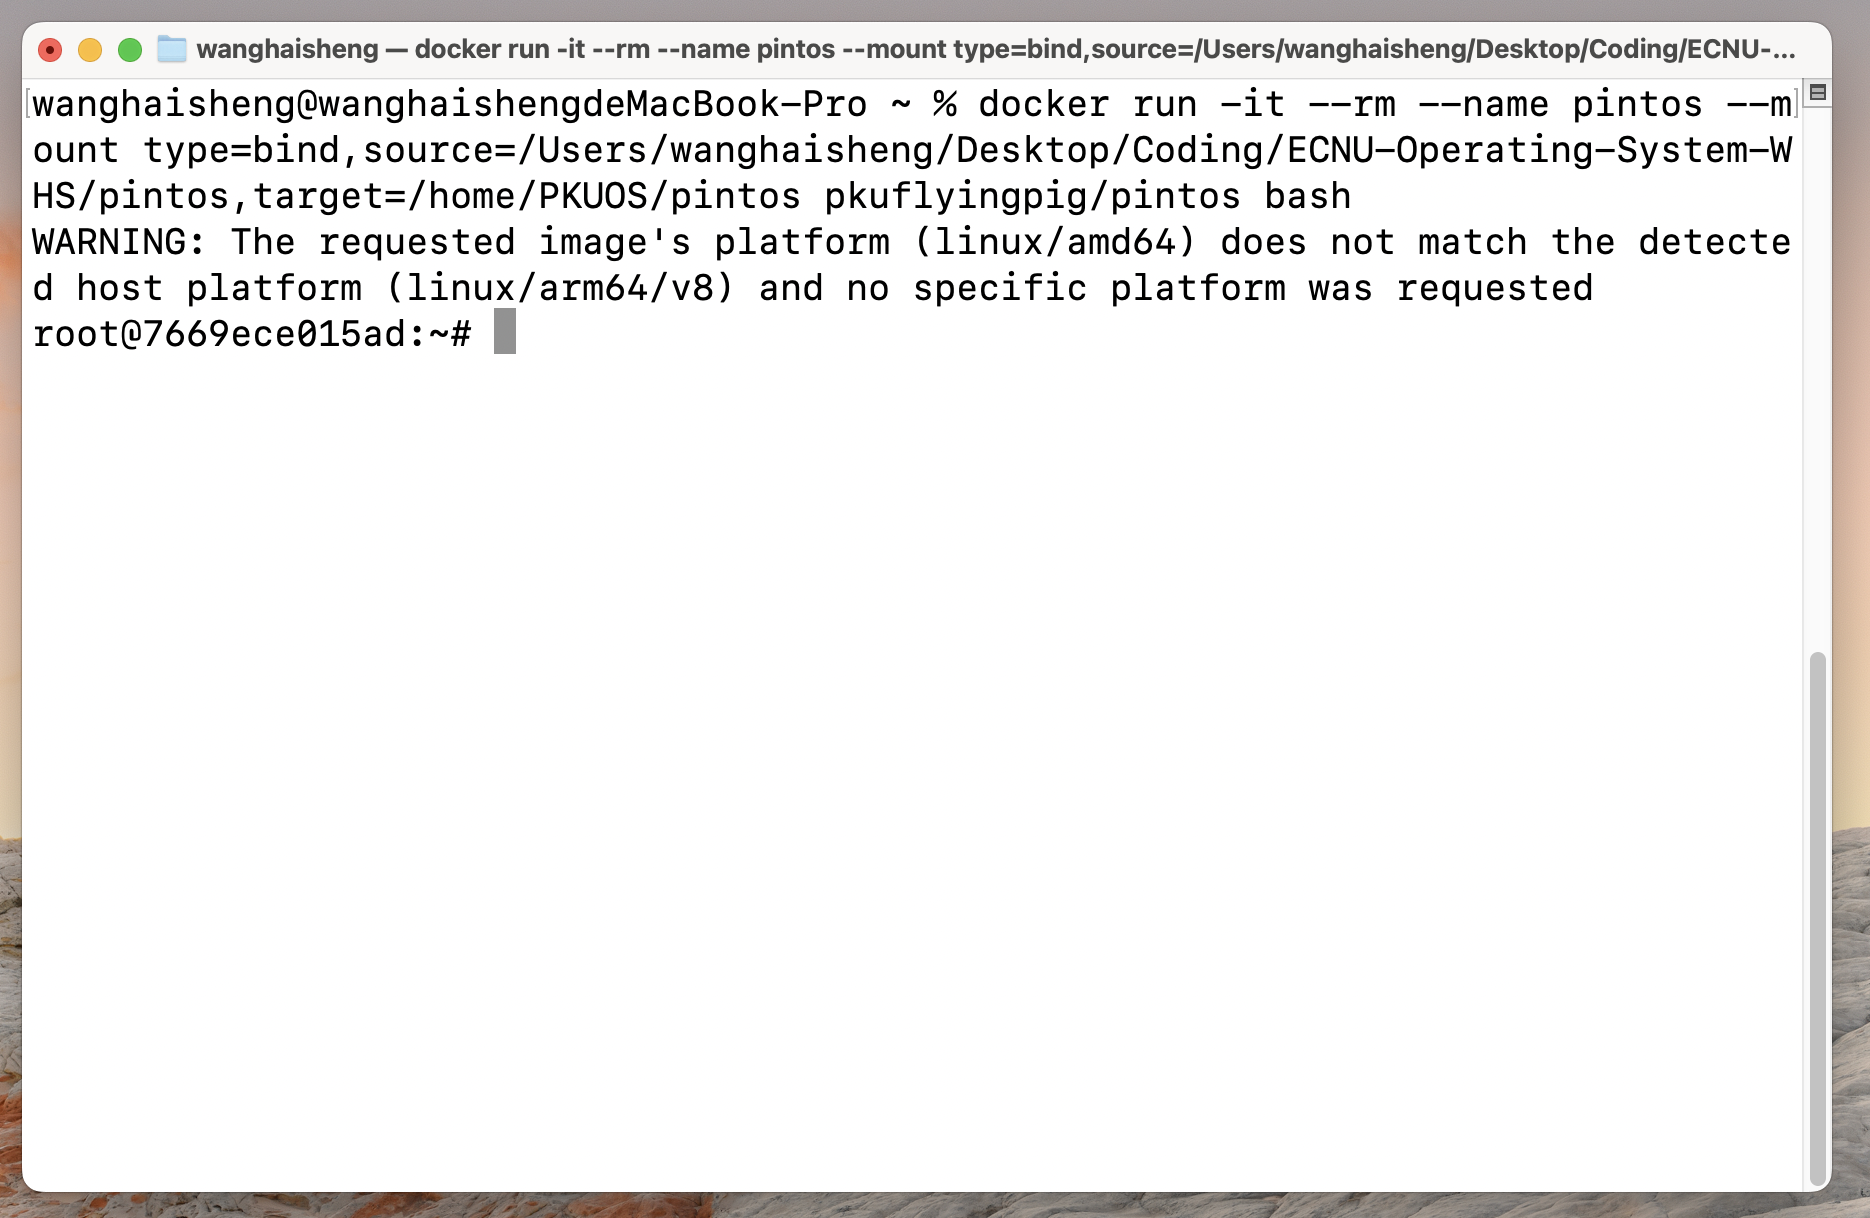
\includegraphics[width=0.9\textwidth]{img/run_docker.png}
	\caption{完成环境配置}
\end{figure}

\normalsize

\section{实验过程}

\normalsize

\section{实验总结}

\normalsize

\section{附录:修改后的代码}

\begin{lstlisting}[language=C, title=\texttt{hello-world.c}]
	#include <stdio.h>
	#include "tests/threads/tests.h"
	
	void test_hello_world(void) {
		printf("hello world!\n");
	}
\end{lstlisting}

\begin{lstlisting}[language=C, title=\texttt{test.c}]
	#include "tests/threads/tests.h"
	#include <debug.h>
	#include <string.h>
	#include <stdio.h>
	
	struct test 
	{
		const char *name;
		test_func *function;
	};
	
	static const struct test tests[] = 
	{
		{"hello-world", test_hello_world},
		{"alarm-single", test_alarm_single},
		{"alarm-multiple", test_alarm_multiple},
		{"alarm-simultaneous", test_alarm_simultaneous},
		{"alarm-priority", test_alarm_priority},
		{"alarm-zero", test_alarm_zero},
		{"alarm-negative", test_alarm_negative},
		{"priority-change", test_priority_change},
		{"priority-donate-one", test_priority_donate_one},
		{"priority-donate-multiple", test_priority_donate_multiple},
		{"priority-donate-multiple2", test_priority_donate_multiple2},
		{"priority-donate-nest", test_priority_donate_nest},
		{"priority-donate-sema", test_priority_donate_sema},
		{"priority-donate-lower", test_priority_donate_lower},
		{"priority-donate-chain", test_priority_donate_chain},
		{"priority-fifo", test_priority_fifo},
		{"priority-preempt", test_priority_preempt},
		{"priority-sema", test_priority_sema},
		{"priority-condvar", test_priority_condvar},
		{"mlfqs-load-1", test_mlfqs_load_1},
		{"mlfqs-load-60", test_mlfqs_load_60},
		{"mlfqs-load-avg", test_mlfqs_load_avg},
		{"mlfqs-recent-1", test_mlfqs_recent_1},
		{"mlfqs-fair-2", test_mlfqs_fair_2},
		{"mlfqs-fair-20", test_mlfqs_fair_20},
		{"mlfqs-nice-2", test_mlfqs_nice_2},
		{"mlfqs-nice-10", test_mlfqs_nice_10},
		{"mlfqs-block", test_mlfqs_block},
	};
	
	static const char *test_name;
	
	/** Runs the test named NAME. */
	void
	run_test (const char *name) 
	{
		const struct test *t;
		
		for (t = tests; t < tests + sizeof tests / sizeof *tests; t++)
		if (!strcmp (name, t->name))
		{
			test_name = name;
			msg ("begin");
			t->function ();
			msg ("end");
			return;
		}
		PANIC ("no test named \"%s\"", name);
	}
	
	/** Prints FORMAT as if with printf(),
	prefixing the output by the name of the test
	and following it with a new-line character. */
	void
	msg (const char *format, ...) 
	{
		va_list args;
		
		printf ("(%s) ", test_name);
		va_start (args, format);
		vprintf (format, args);
		va_end (args);
		putchar ('\n');
	}
	
	/** Prints failure message FORMAT as if with printf(),
	prefixing the output by the name of the test and FAIL:
	and following it with a new-line character,
	and then panics the kernel. */
	void
	fail (const char *format, ...) 
	{
		va_list args;
		
		printf ("(%s) FAIL: ", test_name);
		va_start (args, format);
		vprintf (format, args);
		va_end (args);
		putchar ('\n');
		
		PANIC ("test failed");
	}
	
	/** Prints a message indicating the current test passed. */
	void
	pass (void) 
	{
		printf ("(%s) PASS\n", test_name);
	}
\end{lstlisting}

\begin{lstlisting}[language=C, title=\texttt{test.h}]
	#ifndef TESTS_THREADS_TESTS_H
	#define TESTS_THREADS_TESTS_H
	
	void run_test (const char *);
	
	typedef void test_func (void);
	
	extern test_func test_hello_world;
	
	extern test_func test_alarm_single;
	extern test_func test_alarm_multiple;
	extern test_func test_alarm_simultaneous;
	extern test_func test_alarm_priority;
	extern test_func test_alarm_zero;
	extern test_func test_alarm_negative;
	extern test_func test_priority_change;
	extern test_func test_priority_donate_one;
	extern test_func test_priority_donate_multiple;
	extern test_func test_priority_donate_multiple2;
	extern test_func test_priority_donate_sema;
	extern test_func test_priority_donate_nest;
	extern test_func test_priority_donate_lower;
	extern test_func test_priority_donate_chain;
	extern test_func test_priority_fifo;
	extern test_func test_priority_preempt;
	extern test_func test_priority_sema;
	extern test_func test_priority_condvar;
	extern test_func test_mlfqs_load_1;
	extern test_func test_mlfqs_load_60;
	extern test_func test_mlfqs_load_avg;
	extern test_func test_mlfqs_recent_1;
	extern test_func test_mlfqs_fair_2;
	extern test_func test_mlfqs_fair_20;
	extern test_func test_mlfqs_nice_2;
	extern test_func test_mlfqs_nice_10;
	extern test_func test_mlfqs_block;
	
	void msg (const char *, ...);
	void fail (const char *, ...);
	void pass (void);
	
	#endif /**< tests/threads/tests.h */
\end{lstlisting}

\begin{lstlisting}[language=Bash, title=\texttt{Make.tests}]
	# -*- makefile -*-
	
	include $(patsubst %,$(SRCDIR)/%/Make.tests,$(TEST_SUBDIRS))
	
	PROGS = $(foreach subdir,$(TEST_SUBDIRS),$($(subdir)_PROGS))
	TESTS = $(foreach subdir,$(TEST_SUBDIRS),$($(subdir)_TESTS))
	EXTRA_GRADES = $(foreach subdir,$(TEST_SUBDIRS),$($(subdir)_EXTRA_GRADES))
	
	OUTPUTS = $(addsuffix .output,$(TESTS) $(EXTRA_GRADES))
	ERRORS = $(addsuffix .errors,$(TESTS) $(EXTRA_GRADES))
	RESULTS = $(addsuffix .result,$(TESTS) $(EXTRA_GRADES))
	
	ifdef PROGS
	include ../../Makefile.userprog
	endif
	
	TIMEOUT = 60
	
	clean::
	rm -f $(OUTPUTS) $(ERRORS) $(RESULTS) 
	
	grade:: results
	$(SRCDIR)/tests/make-grade $(SRCDIR) $< $(GRADING_FILE) | tee $@
	
	check:: results
	@cat $<
	@COUNT="`egrep '^(pass|FAIL) ' $< | wc -l | sed 's/[ 	]//g;'`"; \
	FAILURES="`egrep '^FAIL ' $< | wc -l | sed 's/[ 	]//g;'`"; \
	if [ $$FAILURES = 0 ]; then					  \
	echo "All $$COUNT tests passed.";			  \
	else								  \
	echo "$$FAILURES of $$COUNT tests failed.";		  \
	exit 1;							  \
	fi
	
	results: $(RESULTS)
	@for d in $(TESTS) $(EXTRA_GRADES); do			\
	if echo PASS | cmp -s $$d.result -; then	\
	echo "pass $$d";			\
	else						\
	echo "FAIL $$d";			\
	fi;						\
	done > $@
	
	outputs:: $(OUTPUTS)
	
	$(foreach prog,$(PROGS),$(eval $(prog).output: $(prog)))
	$(foreach test,$(TESTS),$(eval $(test).output: $($(test)_PUTFILES)))
	$(foreach test,$(TESTS),$(eval $(test).output: TEST = $(test)))
	$(foreach test,$(TESTS),$(eval $(test).result: $(test).output $(test).ck))
	
	# Prevent an environment variable VERBOSE from surprising us.
	VERBOSE =
	
	TESTCMD = pintos -v -k -T $(TIMEOUT)
	TESTCMD += $(SIMULATOR)
	TESTCMD += $(PINTOSOPTS)
	ifeq ($(filter userprog, $(KERNEL_SUBDIRS)), userprog)
	TESTCMD += $(FILESYSSOURCE)
	TESTCMD += $(foreach file,$(PUTFILES),-p $(file) -a $(notdir $(file)))
	endif
	ifeq ($(filter vm, $(KERNEL_SUBDIRS)), vm)
	TESTCMD += --swap-size=4
	endif
	TESTCMD += -- -q
	TESTCMD += $(KERNELFLAGS)
	ifeq ($(filter userprog, $(KERNEL_SUBDIRS)), userprog)
	TESTCMD += -f
	endif
	TESTCMD += $(if $($(TEST)_ARGS),run '$(*F) $($(TEST)_ARGS)',run $(*F))
	TESTCMD += < /dev/null
	TESTCMD += 2> $(TEST).errors $(if $(VERBOSE),|tee,>) $(TEST).output
	%.output: kernel.bin loader.bin
	$(TESTCMD)
	
	%.result: %.ck %.output
	perl -I$(SRCDIR) $< $* $@
\end{lstlisting}

\begin{lstlisting}[language=Bash, title=\texttt{hello-world.ck}]
	# -*- perl -*-
	use strict;
	use warnings;
	use tests::tests;
	check_expected([<<'EOF']);
	(hello-world) begin
	hello world!
	(hello-world) end
	EOF
	pass;
\end{lstlisting}

\normalsize

\end{document}